\documentclass[../main.tex]{subfiles}

\begin{document}
\section{Task 2 -- ANN-UTADIS}

The trained model heavily utilised code provided in \verb|ANN-UTADIS.ipynb| and \verb|helpers.py|.
Small changes were introduced to suit the authors' preferences better, but the overall
architecture is based entirely on these snippets.
The model analysed in this section contains 12 hidden layers.

It is essential to note here that the two cost type criteria: \emph{buying} and \emph{maint}
have been transformed in the following way:
\verb|new_value = 1 - old_value|.
Thanks to this procedure more preferred values are represented by larger numbers,
just as in the case of gain type criteria.
This is done in order to facilitate using non-decreasing marginal value functions for all criteria.
\subsection{Model visualization}
\begin{figure}[H]
    \centering
    \begin{subfigure}[b]{0.48\linewidth}
        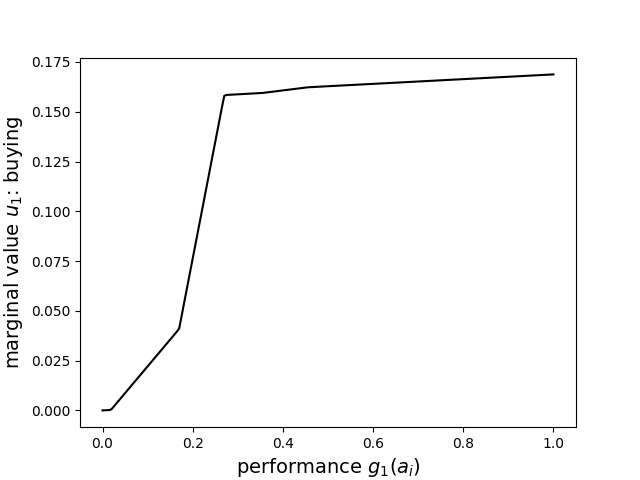
\includegraphics[width=\linewidth]{../img/marginal0.png}
    \end{subfigure}
    \begin{subfigure}[b]{0.48\linewidth}
        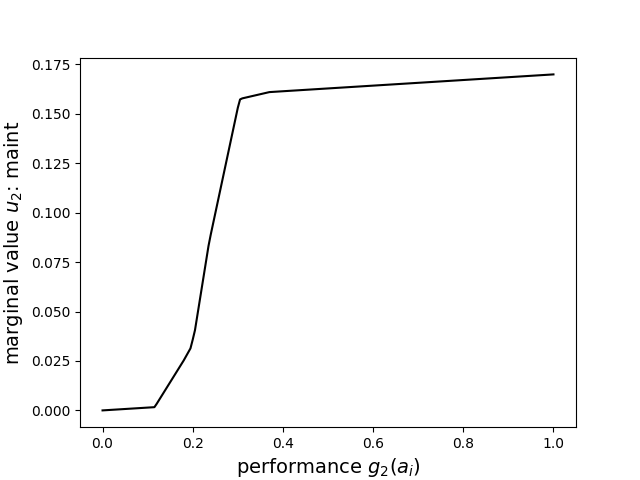
\includegraphics[width=\linewidth]{../img/marginal1.png}
    \end{subfigure}

    \begin{subfigure}[t]{0.48\linewidth}
        \makeatletter\def\@currentlabel{plot}\makeatother
        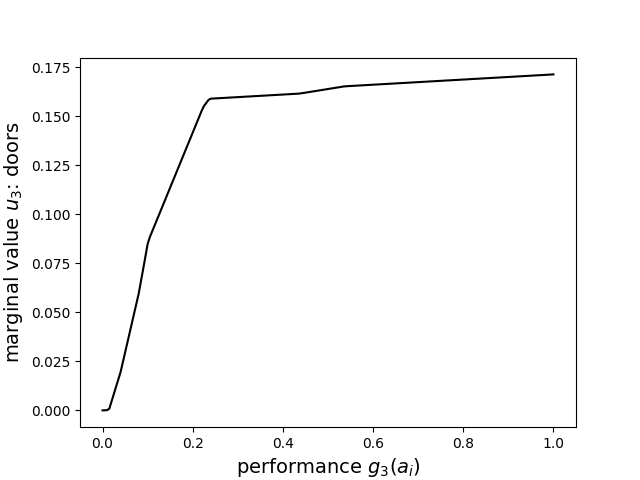
\includegraphics[width=\linewidth]{../img/marginal2.png}
        \label{fig:UTA-marginal-doors}
    \end{subfigure}
    \begin{subfigure}[b]{0.48\linewidth}
        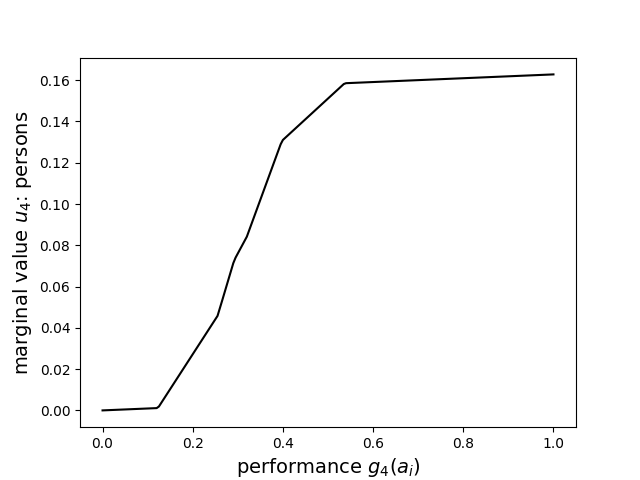
\includegraphics[width=\linewidth]{../img/marginal3.png}
    \end{subfigure}
    \end{figure}

    \begin{figure}\ContinuedFloat
    \begin{subfigure}[b]{0.48\linewidth}
        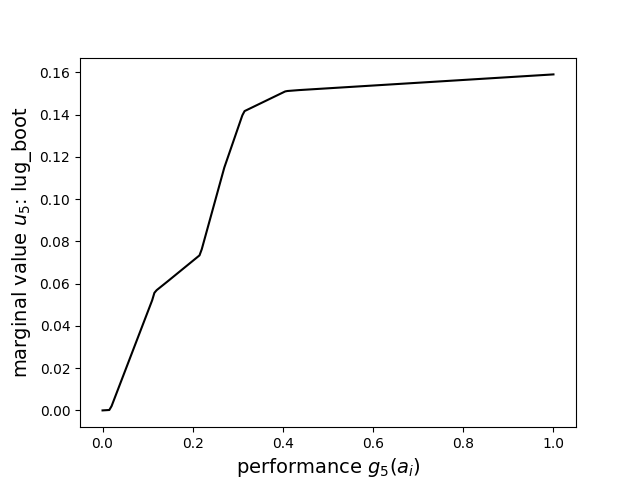
\includegraphics[width=\linewidth]{../img/marginal4.png}
    \end{subfigure}
    \begin{subfigure}[b]{0.48\linewidth}
        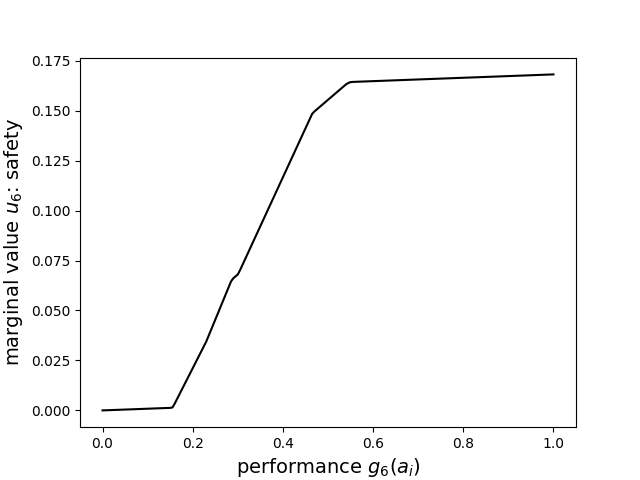
\includegraphics[width=\linewidth]{../img/marginal5.png}
    \end{subfigure}
    \caption{Marginal value functions for all criteria generated by the network}
\end{figure}

\begin{figure}[H]
    \centering
    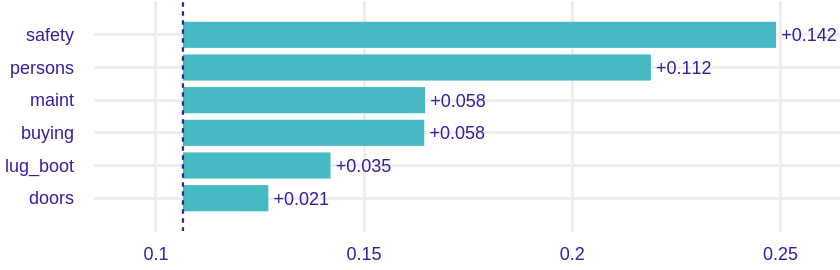
\includegraphics[width=\linewidth]{../img/UTA-feature-importance.png}
    \caption{ANN-UTADIS feature importance as computed by DALEX}
    \label{fig:UTA-feats}
\end{figure}

\subsection{Preference analysis}

% Based on the parameters obtained, can we say something about the user’s
% preferences? Are there any criteria that have no effect, or have a decisive
% influence? Whether there are any preference thresholds? Are there any
% evaluations on criteria that are indifference in terms of preferences?
The UTA model has the advantage that it utilises marginal preference functions,
which can be very directly interpreted as an expression of DM's preference.
Looking at them, no criterion seems to have a decisive influence or be irrelevant.
The maximum values of their marginal value functions ("weights")
are very similar - they are all concentrated roughly between 0.16 and 0.18.

All but one functions are more or less flat for larger values of $g_i$, suggesting
that the decision maker is rather indifferent regarding whether an alternative is
exceptional on one criterion. In other words, the DM is interested in balanced alternatives.
This claim is reinforced by the results of ceteris paribus analysis -
changing the value of just one parameter never has a significant effect on
the model's overall prediction.

An especially interesting marginal value function is the one regarding criterion $u_2$ \emph{doors}.
Having 3 doors seems to be a very big advantage over having only 2,
but adding more doesn't give much benefit, as seen on  its \ref{fig:UTA-marginal-doors}.
This is also reflected in the ceteris paribus plots discussed later.

The feature importance plot generated by DALEX is significantly less uniform. \emph{doors} seems
yet again to be the most interesting attribute, with its low importance. I think that this
might be because a large range of performance values result in almost no change in
the value of $u_i$.
\subsection{3-alternative analysis}

\subsubsection{Analytical approach}
We can use the marginal value functions to get an insight into how the model
performs classification. The model would assign an object to a different class if
their sum (comprehensive value) is smaller than 0.5. Based on that we can make the
following inferences:
- \emph{best} can't be classified as unacceptable by changing the value on just one criterion
- \emph{worst} can't be classified as acceptable by changing the value on just one criterion

For \emph{mid}, things are a bit more complicated. As is, it is assigned 0 (unacceptable).
However, it attains the maximum possible score for \emph{buying}, \emph{maint}, and \emph{lug\_boot}.
It's 0.5 on \emph{persons} should already give it most of the "score" from this criterion, so improvement
should be sought elsewhere. We are left with \emph{doors} and \emph{safety}, which are originally at 0 for \emph{mid}.
I suspect, that changing \emph{doors} to 0.25 could be enough.
It should certainly do more than adding the same value to \emph{safety}, due to the sharper increase of the
marginal value function of the former. Running the model for such two alternatives confirms this assessment.
With \emph{doors} = 0.25, the model classifies the alternative as barely acceptable with 0.0009,
while changing \emph{safety} to 0.25 maintains negative judgement with -0.1128

\subsubsection{Space sampling}
To concisely show how changing the value of just one attribute would change the result, ceteris paribus analysis
was performed.

Files with all plots are available in \verb`report/img/extras`. In order not to overcrowd the report,
only the plots for \emph{doors} for the 3 alternatives are presented.

\begin{figure}[H]
    \centering
    \begin{subfigure}[b]{0.4\linewidth}
        \makeatletter\def\@currentlabel{DALEX plot}\makeatother
        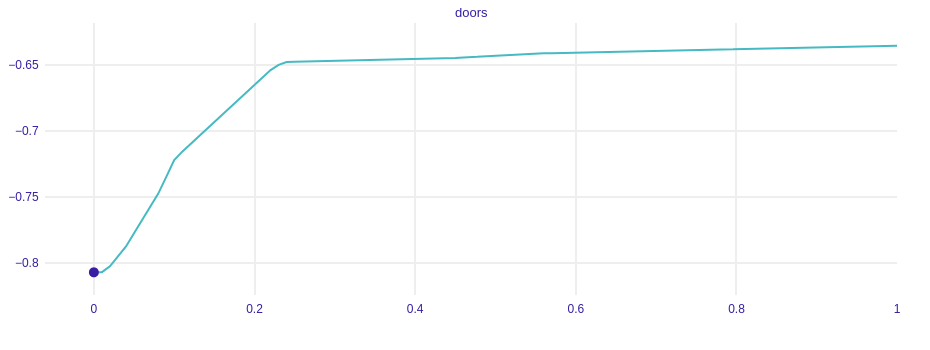
\includegraphics[width=\linewidth]{../img/doors_worst.png}
        \label{fig:UTA-ceteris-paribus-doors}
    \end{subfigure}
    \begin{subfigure}[b]{0.4\linewidth}
        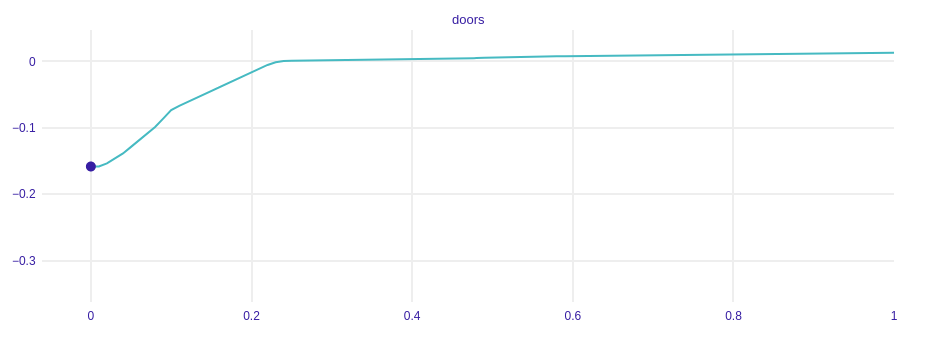
\includegraphics[width=\linewidth]{../img/doors_medium.png}
    \end{subfigure}

    \begin{subfigure}[b]{0.4\linewidth}
        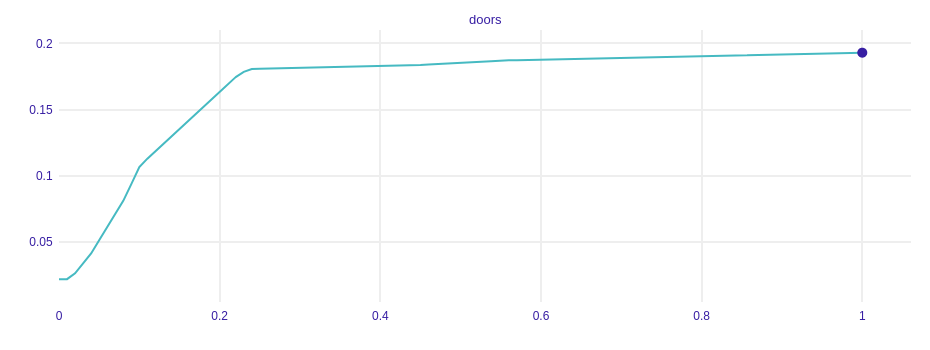
\includegraphics[width=\linewidth]{../img/doors_best.png}
    \end{subfigure}
    \caption{Ceteris paribus analysis for criterion \emph{doors} for (from left to right and
    top to bottom)}
\end{figure}

In image form, the plots can't be examined as thoroughly as in interactive DALEX output, but it agreed
with the earlier theoretical prediction, and measured model output. It showed that \emph{doors}=0.25 would result
in \emph{mid} being classified as acceptable. It also allows us to see, that with \emph{doors}=0.23, the
model is expected to produce -0.001, but that changing the value of this attribute to 0.24 might be sufficient to
obtain a positive result.

\subsubsection{Variable contribution plots}
\begin{figure}[H]
    \centering
    \begin{subfigure}{0.78\linewidth}
        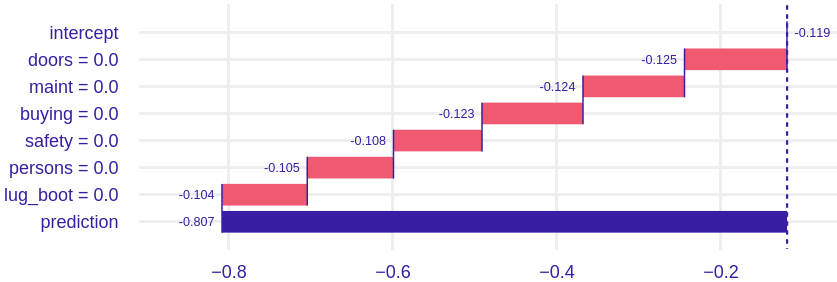
\includegraphics[width=\linewidth]{../img/UTA-breakdown-worst.png}
        \caption{Variable contribution of alternative 1 (worst) in ANN-UTADIS}
        \label{fig:UTA-3alt1-contrib}
    \end{subfigure}
    \begin{subfigure}{0.78\linewidth}
        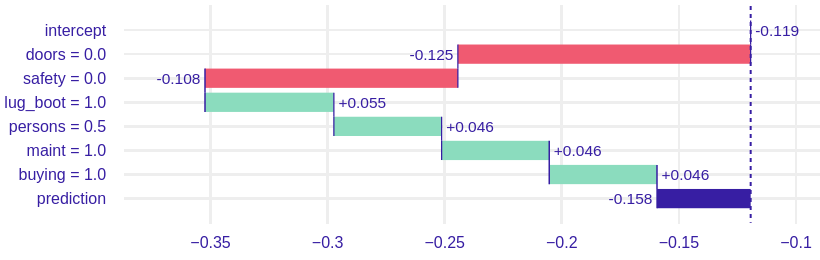
\includegraphics[width=\linewidth]{../img/UTA-breakdown-mid.png}
        \caption{Variable contribution of alternative 2 (mid) in ANN-UTADIS}
        \label{fig:UTA-3alt2-contrib}
    \end{subfigure}\end{figure}
    \begin{figure}[H]\ContinuedFloat
    \centering
    \begin{subfigure}{0.78\linewidth}
        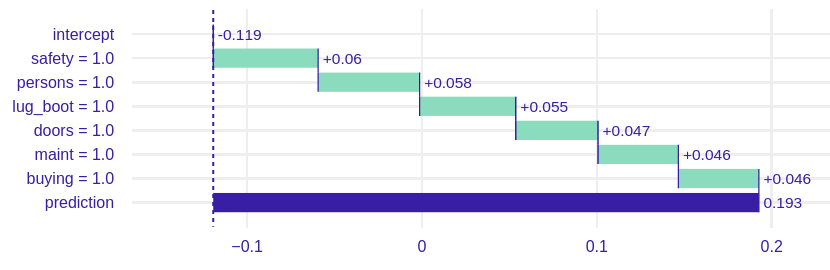
\includegraphics[width=\linewidth]{../img/UTA-breakdown-best.png}
        \caption{Variable contribution of alternative 3 (best) in ANN-UTADIS}
        \label{fig:UTA-3alt3-contrib}
    \end{subfigure}
\end{figure}

\end{document}
